\section{Teoria della relatività ristretta}
    \subsection{Sistemi di riferimento inerziali e principio di relatività di Galileo}
        \par Si definisce sistema di riferimento inerziale un sistema nel quale un corpo non subisce forze per effetto del moto del sistema stesso
        \par In buona approssimazione possiamo considerare la Terra come se fosse un sistema di riferimento inerziale; tutti i sistemi di riferimento in moto relativo uniforme rispetto alla Terra, di conseguenza, sono sistemi di riferimento inerziali.
        \par Convenzionalmente consideriamo due sistemi di riferimento inerziali $Oxy$ e $O'x'y'$ con gli assi $x$ e $x'$ paralleli e le origini coincidenti a $t=0$. $O'$ si muove a $\vec{V}_rel$ rispetto a $O$ e $\vec{u}$ è la velocità di un corpo rispetto ad $O$, mentre $\vec{u}'$ è la velocità rispetto a $O'$.
        \par Scriviamo le trasformazioni di Galileo per la posizione, la velocità e l'accelerazione di un corpo fra un sistema di riferimento e un altro.
        \subsubsection{Equazioni per la posizione}
        \begin{equation}
            \begin{cases}
            x = x' + V_{rel}^x(t)\\
            y = y'\\
            z = z'
            \end{cases}
        \end{equation}
        \subsubsection{Equazioni per la velocità}
        \begin{equation}
            \begin{cases}
            v_x = v_x' + V_{rel}^x\\
            v_y = v_y'\\
            v_z = v_z'
            \end{cases}
        \end{equation}
        \subsubsection{Equazioni per l'accelerazione}
        \begin{equation}
            \begin{cases}
            a_x = a_x'\\
            a_y = a_y'\\
            a_z = a_z'
            \end{cases}
        \end{equation}
        \par \textbf{Principio di relatività di Galileo}: le leggi della meccanica sono uguali in tutti i sistemi di riferimento inerziali.
        \subsubsection{Osservazioni sulle trasformazioni di Galileo}
        \par Il tempo non viene preso in considerazione nelle trasformazioni poiché si dava per scontato che osservatori inerziali diversi misurassero la distanza temporale fra due eventi in maniera identica.
        \par Quest'approccio, benché intuitivo, non è scientificamente corretto in quanto manca la verifica sperimentale
    \subsection{Analisi del concetto di simultaneità di due eventi}
        \par Per indicare un evento bisogna fornire tre coordinate spaziali ($x$, $y$ e $z$) ed una coordinata temporale t.
        \par La distanza temporale fra due eventi viene chiamata durata temporale ed indicata con ${\Delta}t$.
        \par \esempio
        \par Evento 1: $E_1(x_1,y_1,z_1,t_1)$
        \par Evento 2: $E_1(x_2,y_2,z_2,t_2)$
        \par ${\Delta}t = t_2-t_1$
        \par Vogliamo vedere come due osservatori inerziali in moto relativo fra loro giudicano due eventi.
        \par Per l'osservatore fermo $O$ i due eventi risultano simultanei. Per l'osservatore $O'$, avente $V_{rel}^x=100 \frac{m}{s}$ e $x'(0)=x(0)$, avverrà prima l'evento a lui più vicino.
        \par Conclusione: la simultaneità di due eventi è relativa: due eventi possono apparire simultanei ad un osservatore inerziale e non simultanei ad un altro osservatore inerziale.
    \subsection{I postulati della relatività ristretta}
        \begin{enumerate}
            \item Le leggi della fisica sono uguali in tutti i sistemi di riferimento inerziali (generalizzazione del principio di relatività di Galileo)
            \item La velocità della luce è la stessa per tutti i sistemi di riferimento inerziali
        \end{enumerate}
        \par Commento: il secondo postulato riprende le conclusioni che si ottengono applicando le equazioni di Maxwell, quindi è in accordo con esse; esso è in palese disaccordo con le trasformazioni di Galileo.
        \par
        \begin{tabular}{p{7.5cm}|p{7.5cm}}
        \textbf{Meccanica classica}                                                                                                    & \textbf{Relatività ristretta}                                                                   \\ \hline
        Principio di relatività di Galileo                                                                                                                   & Principio di relatività di Einstein                                                                                  \\
        La velocità della luce cambia al variare della velocità dell'osservatore inerziale, in accordo con quanto prescritto dalle trasformazioni di Galileo & $c$ è costante per tutti i sistemi di riferimento inerziali. Questa ipotesi è in accordo con le equazioni di Maxwell \\
        Postulato implicito: ${\Delta}t={\Delta}t'$                                                                                                          & ${\Delta}t$=?                                                                                                        \\
        $\vec{a}=\frac{\vec{F}_{tot}}{m}$                                                            &                                                                                                                     
        \end{tabular}
    \subsection{Intervallo di tempo proprio e dilatazione dei tempi}
        \par Si definisce sistema di riferimento proprio per un certo fenomeno fisico il sistema di riferimento nel quale fenomeno stesso inizia e finisce nello stesso punto.
        \par La durata del fenomeno fisico in tale sistema di riferimento proprio viene chiamato intervallo di tempo proprio ($\Delta\tau$). In meccanica classica si da per scontato che l'intervallo di tempo proprio $\Delta\tau$ e l'intervallo di tempo non proprio misurato da un qualsiasi osservatore non proprio siano uguali.
        \par Determiniamo la relazione fra un intervallo di tempo proprio per un certo fenomeno e il corrispondente intervallo di tempo non proprio misurato da un osservatore non proprio, nell'ipotesi che $c$ sia costante.
        \par Immaginiamo di considerare il fenomeno fisico del viaggio di un raggio di luce dal tavolino di un treno al soffitto e viceversa.
        % \begin{figure}[h]
        %     \caption{Nella figura a sinistra è rappresentato il fenomeno dal punto di vista di un osservatore non proprio esterno al treno, mentre nella figura a destra è rappresentato il punto di vista dell'osservatore proprio}
        %     \centering
        %     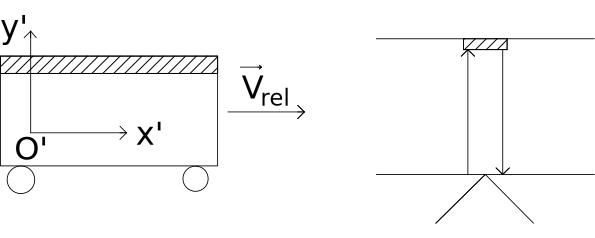
\includegraphics[width=15cm]{res/53reltempo}
        % \end{figure}
        \par Indichiamo con $\Delta\tau$ l'intervallo di tempo proprio misurato dall'osservatore proprio sul treno ($\Delta\tau=\frac{2d}{c}$). Analizziamo lo stesso fenomeno dal punto di vista dell'osservatore $O'$ fermo a terra.
        % \begin{figure}[h]
        %     \caption{Dettaglio del fenomeno visto da terra}
        %     \centering
        %     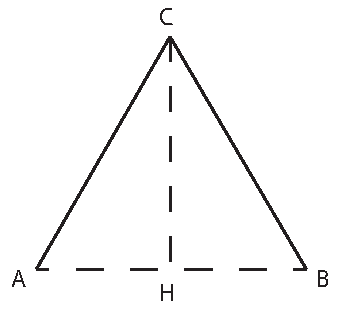
\includegraphics[width=15cm]{res/53reltempo2}
        % \end{figure}
        \begin{equation*}
            AC^2=AH^2+CH^2
        \end{equation*}
        \begin{equation*}
            (\frac{1}{2}c\cdot\Delta t)^2 = (\frac{1}{2}V_{rel}\Delta t)^2 + (\frac{1}{2}c\Delta\tau)^2
        \end{equation*}
        \begin{equation*}
            c^2\Delta{t}^2=V_{rel}^2\Delta{t} + c^2\Delta\tau2
        \end{equation*}
        \begin{equation*}
            \Delta{t}^2(c^2-V_{rel}^2) = \Delta{t}^2(1-\frac{V_{rel}^2}{c^2})
        \end{equation*}
        \begin{equation*}
            \Delta{t}=\Delta\tau\cdot\frac{1}{\sqrt{1-\frac{V_{rel}^2}{c^2}}}
        \end{equation*}
        \par Poniamo $\gamma=\frac{1}{\sqrt{1-\frac{V_{rel}^2}{c^2}}}$ e notiamo che $\gamma \geq 1 \forall V_{rel} \in \mathbb{R}$. Otteniamo che
        \begin{equation}\label{eq:53reltempi}
            \Delta{t} = \gamma\Delta\tau
        \end{equation}

